\begin{figure}
\begin{center}
    \centering
    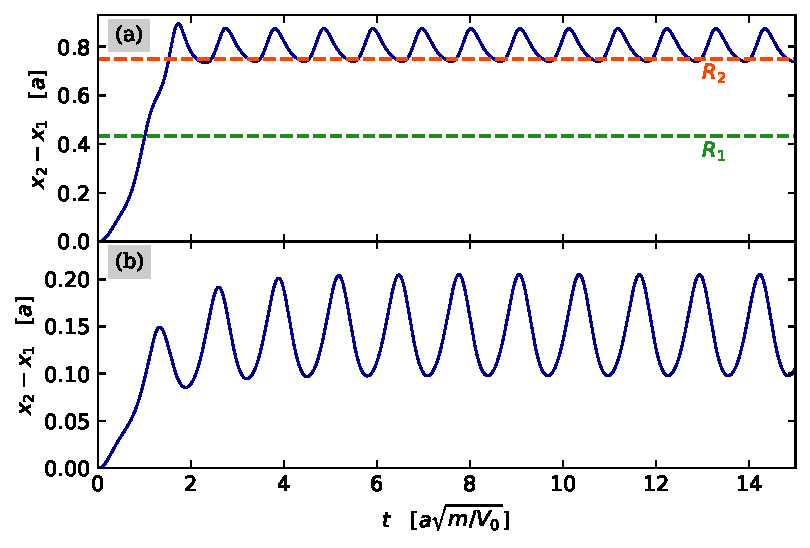
\includegraphics[width=1\linewidth]{Images/different.pdf}
    \caption{Oscillations with different damping factors for the two particles. $R_1 = \frac{\sqrt{3}}{4} a$, $R_2 = 0.75 a$, $ U = 10 \p$ (and therefore $\delta = 0.2637 V_0$), $F = 7.5 \f$, $\gamma_1 = 10 \g$ and initial condition $R_0=0$. \textbf{(a)} $\gamma_2 = 0.5 \gamma_1$; \textbf{(b)} $\gamma_2 = 0.8 \gamma_1$.  }
    \label{Fig:different}
\end{center}
\end{figure}

In this section we study how the system changes when the symmetry between the two particles $x_1$ and $x_2$ is broken, by taking two different damping factors that we call $\gamma_1$ and $\gamma_2$, respectively. This means that now the units forming the molecule are different, as could occur in a real physical system. 

For simplicity, we fix the damping factor of the first particle $\gamma_1$ to $10\g$, investigating what happens when $\gamma_2$ is smaller, but always remaining in the overdamped regime. With such a system, we expect the particle with the smaller damping factor, $x_2$, to move with more ease when dragged trough the corrugation of $V_{ext}$, and thus to remain ahead of the first particle. This is confirmed by the oscillations reported in Fig.~\ref{Fig:different}. In Fig.~\ref{Fig:different}a, we take $\gamma_2 = 0.5 \gamma_1$. With such a large difference in the damping factors, $r$ moves rapidly to $R_2$ even with the initial condition $R_0 = 0$. As can be seen, for sufficiently large driving force F, eventually $r$ oscillates around a point beyond $R_2$. In Fig.~\ref{Fig:different}b, the difference in the damping factors is smaller, setting $\gamma_2 = 0.8\gamma_1$. For the same applied force, if $r$ starts from the origin, it does not overcome the potential barrier at $R_1$. This does not imply that the molecule remains collapsed at the origin. Instead, a small-amplitude oscillation is established around a point $r>0$. A similar oscillation is found also in the previous case of $\gamma_2 = 0.5\gamma_1$, but only for greater values of the potential barrier $\delta$, that can eventually prevent $r$ from reaching the second minimum.

%The effects of different gammas is that of effectively adding a force $F_{eff} = m(\gamma_1 - \gamma_2)\dot{x}_1$ to the Eq.~\eqref{eq:rdot} for $r$. To the extent that $\dot{x}_1 \approx \Bar{v}_\text{cm}$, this constant force can be described as an additional conservative term in the potential $\Tilde{V} = -F_{eff}\cdot r$. The addition of this linear term determines a displacement to the right of the minima of $V_\text{int} + \Tilde{V}$, both the one near the origin and the one near $R_2$. The larger the difference between $\gamma_1$ and $\gamma_2$ is, the further these new minima are shifted to the right.

Allowing two different damping factors for the two particles, Eq.~\eqref{eq:rdot} modifies as follows:
\begin{equation}
    \mu\ddot{r} = -\frac{V_0\pi}{a}\cos \left(\frac{2\pi x_\text{cm}}{a}\right)\sin\left(\frac{\pi r}{a}\right)
    - V'_\text{int}(r) -2\mu\Bar{\gamma}\dot{r}+2\mu\gamma_\text{rel}\dot{x}_\text{cm},
    \label{eq:diff}
\end{equation}
where $\Bar{\gamma} = (\gamma_1+\gamma_2)/2$ and $\gamma_\text{rel} = \gamma_1-\gamma_2$.
Comparing Eq.~\eqref{eq:rdot} with Eq.~\eqref{eq:diff}, we can identify the damping factor of the internal molecular motion with the mean damping factor $\Bar{\gamma}$. To the extent that $\dot{x}_\text{cm} \approx \Bar{v}_\text{cm}$, the last term of Eq.~\eqref{eq:diff} can be regarded as an additional constant force proportional the difference between the damping factors $\gamma_\text{rel}$. This constant force can be described as an additional conservative term in the potential $\Tilde{V} = -rF_\text{eff}$. The addition of this linear term determines a displacement to the right of the minima of $V_\text{int} + \Tilde{V}$, both the one near the origin and the one near $R_2$. The larger the difference between $\gamma_1$ and $\gamma_2$ is, the further these new minima are shifted to the right. If $F^\text{eff}$ is large enough, the minimum at the origin can eventually be erased, as is in the case reported in Fig.~\ref{Fig:different}a. 